\documentclass[fleqn,10pt]{wlscirep}
\usepackage[utf8]{inputenc}
% \usepackage[style = ieee]{biblatex}
\usepackage[T1]{fontenc}

\usepackage{subfiles}
\usepackage{tikz}
\usepackage{subtikzpicture}

% \usepackage{natbib}
% \usepackage[style=nature]{biblatex}
\title{TinyML in Agriculture Sector: Awakening of Minds in Low Power Edge Devices}

\author[]{Daniel V Mathew}
% \author[1,2,+]{Christine Author}
% \author[2,+]{Derek Author}
\affil[]{Department of Electronics and Communication, Rajiv Gandhi Institute of Technology, Kottayam, 686501, India}

% \affil[*]{danielvmathew27@gmail.com}
%
% \affil[+]{these authors contributed equally to this work}

% \keywords{Antena, Wifi, Pentagonal}

\keywords{TinyML, Agriculture, Smart-farming}

\begin{abstract}

    %% Say about TinyML

    TinyML is a subset of machine learning (ML) that focuses on developing and deploying
    ML models on resource-constrained devices such as Microcontrollers (MCUs), System-on-Chip
    (SoCs) and other such devices. Frameworks such as TensorFlow Lite Micro, and Arm CMSIS-NN
    are used for developing ML models for low powered devices. Techniques used in TinyML
    enables these devices to be more efficient at running ML models. Thereby improving
    decision-making, reducing cost and power consumption.

    %% Say about seminar

    This seminar aims to explore recent trends and advancements in TinyML, specifically in its role in the
    Agriculture sector. TinyML enables low powered devices such as ESP32 CAM modules, STM32
    microcontrollers, and Arduinos to be used in ML applications. These devices can then
    perform growth monitoring, plant disease detection, and mirco-climate management in
    place of expensive Raspberry Pis and other Mini PCs. Thus, TinyML powered low power
    edge devices may find applications in smart agriculture in isolated places and also where
    low power consumption is at top priority.



% The microstrip patch antennas are light weight, low profile can be easily fabricated, planar in
% configuration and can be printed directly on to circuit boards. The scientific software for
% antenna design is High Frequency Structural Simulator (HFSS). By using planar antennas the
% cost can be minimized and can easily fabricated. The tool HFSS is very powerful tool in RF
% domain especially for designing antennas/filters/Three dimensional structures and all other
% active/passive systems.

% In this seminar, a pentagonal patch antenna with
% loaded open loop resonator (OLR) for improvement of gain and
% reduced cross polarization is studied. The standard pentagonal
% patch antenna is taken as the parent structure and further
% improvement in performance characteristics could be  achieved by
% loading the resonator material above the standard pentagonal
% patch antenna.  This antenna may
% finds applications in long range Wi-Fi communications.

\end{abstract}
\begin{document}

\flushbottom
\maketitle
% * <john.hammersley@gmail.com> 2015-02-09T12:07:31.197Z:
%
%  Click the title above to edit the author information and abstract
%
\thispagestyle{empty}

% \noindent Please note: Abbreviations should be introduced at the first mention in the main text – no abbreviations lists. Suggested structure of main text (not enforced) is provided below.

\section*{Background}
\label{sec:background}

    TinyML is a subset of machine learning (ML) that focuses on developing and deploying
    ML models on resource-constrained devices such as Microcontrollers (MCUs), System-on-Chip
    (SoCs) and other such devices. TinyML consists of techniques, and design methodologies
    that improve the efficiency of ML models. This is achieved through \emph{model compression},
    and making use of \emph{efficient algorithms} and \emph{hardware accelerators}.
    Model compression can be achieved via techniques like \emph{pruning}, \emph{quantization},
    and \emph{knowledge distillation}. Use of \emph{optimized ML algorithms} for low-power, low-memory devices
    and utilizing \emph{hardware accelerators} can also help in speeding up the computation.
    The design flow is depicted in Fig. \ref{fig:designFlow}.

% Microstrip patch antennas offer advantages such as light weight, compact size, planar configuration,  ease of fabrication and compatibility with PCB technology \cite{iftissane2011conception}. Various geometries of radiating patch elements such as square, circle, and rectangle have been considered in the previous studies\cite{gupta2013circularly}. However,  microstrip patch antennas generally have narrow bandwidth, low efficiency  due to dielectric and conductor losses and disability to operate at high power levels of waveguide \cite{zhang2016design}\cite{harish20153}\cite{vaishnavi2014simulation}\cite{anand2015analysis}.  The design approach is depicted in Fig. \ref{fig:design}.
%

\begin{figure} [h]
    \centering
    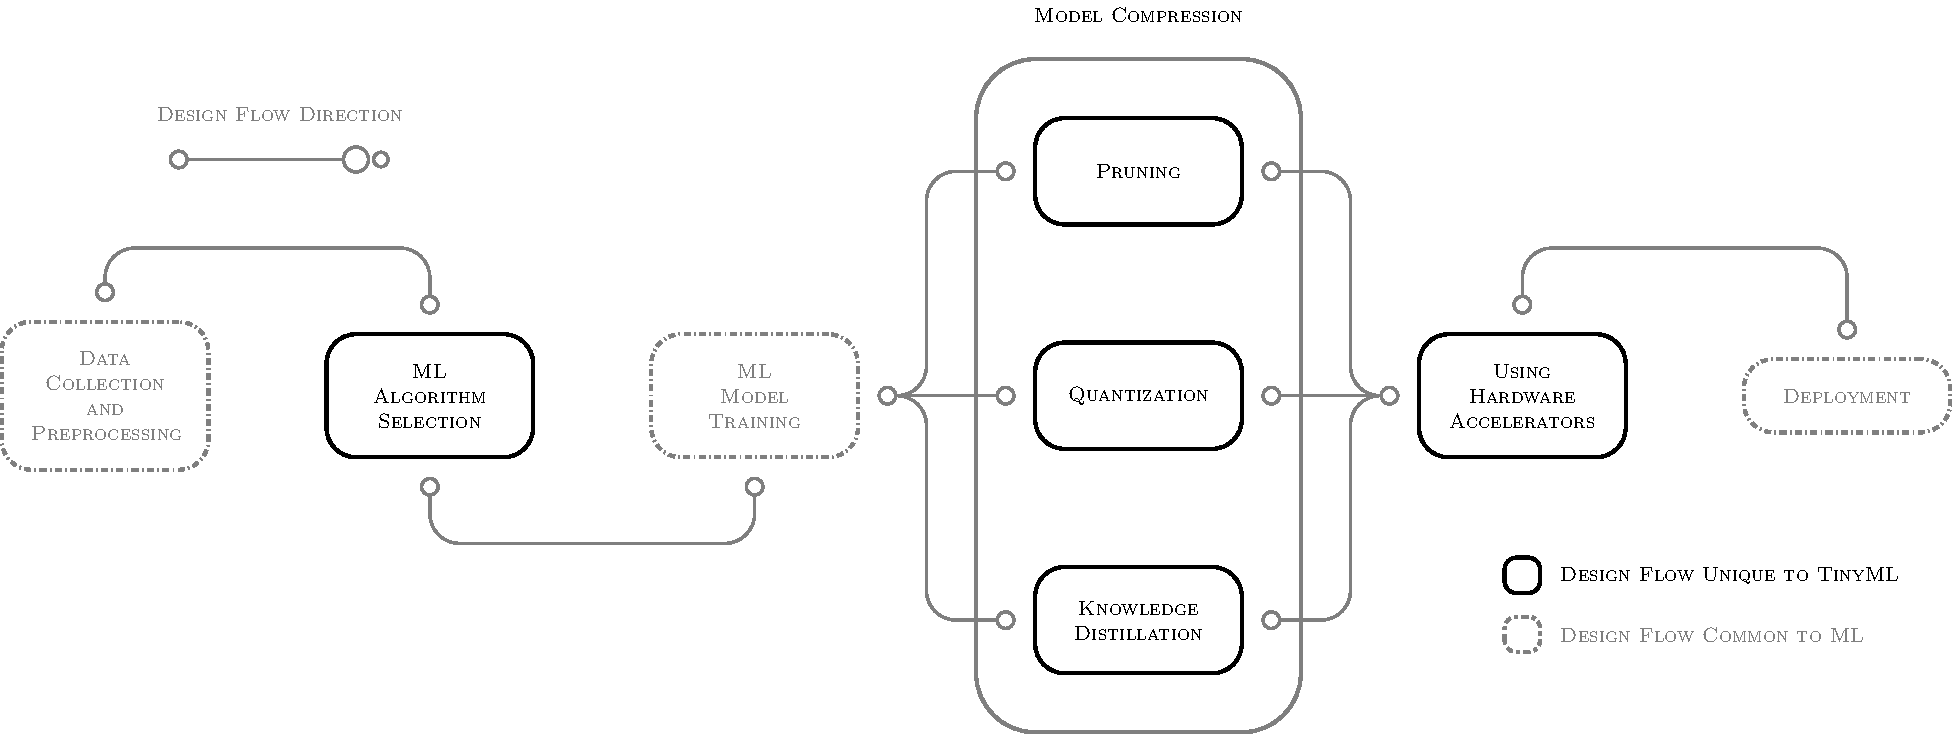
\includegraphics [
        width = 0.95\textwidth,
    ] {tikzpics/endDesignFlow.pdf}
    \captionof{figure} {Typical TinyML Design Flow.}
    \label{fig:designFlow}
\end{figure}



% \begin{figure} [h]
%  \begin{center}
% \label{fig:design}
%  \includegraphics[width=4.0in]{example-image-b}
%  \caption{Design Approach}
%  \label{fig:design}
%  \end{center}
% \end{figure}


\section*{Related Work}
\label{sec:relatedwork}


% \cite{sp00}.

% \nocite{ieee00, ieee01, ieee02, ieee03, ieee04, sd00, sd01}

A real time environmental monitoring system driven by a TinyML model using Graph Neural Network (GNN) optimized with Q learning was proposed\cite{ieee00gnn}
and the system was proven to be better than conventional monitoring systems.
A system based on TinyML for plant disease detection was implemented in the remote areas within West Africa\cite{ieee01africa}. The
study compared the TinyML based system to a cloud based one and found that the TinyML based one had promising performance as
there is no need for internet connectivity.
As per the study\cite{ieee03} conducted, TinyML systems are shown to be ideal choice for detecting the fruit presence in crops.
TinyML systems are also shown to be effective in disease detection as per the studies\cite{sd00, ieee01africa} conducted.
TinyML oriented deep learning model for an intelligent greenhouse microclimate was developed as part of a study\cite{sp02}.
A TinyMlaaS (TinyML as a Service) architecture for future IoT developments was proposed\cite{ieee05}.
A model was developed using Tensorflow Lite for object detection making use of constrained resources on a STM32 microcontroller\cite{sd02}.
Image processing capabilities of TinyML are also backed by further studies\cite{sd03}.
A recent comprehensive survey\cite{ieee06} conducted on TinyML explores the application for low-profile devices.


% A pentagonal patch antenna with loaded open loop resonator (OLR) for enhancing the gain and reducing cross-polarization compared to \cite{lafmajani2011miniaturized}\cite{gupta2019design} is proposed. The intended application of the proposed antenna is a technology for providing internet connectivity to fishermen in deep sea using long range Wi-Fi communications \cite{rao2016realizing}\cite{jayakrishnan2018effect}. The specifications of the antenna required for this application are compact size, high gain for providing required connectivity from shore. Directional antennas providing high gain will enable us to achieve high signal to noise ratio such that connectivity in the order of tens of kilometer can be established. Antenna array solutions, on the other hand, although enhances the gain, but will consume large area and hence not suitable for this application. In the proposed antenna configuration, an inset-fed pentagonal microstrip antenna is taken as the parent structure and performance characteristics are studied. The size of the proposed antenna configuration is much less as compared to conventional antennas of similar gain \cite{joshi2011metamaterial}.


% \bibliographystyle{acm}
\bibliography{References}

\end{document}
